\chapter{Soft Materials Modelling: Linear Viscoelastic Models} \label{sec:ChapterModellingLVM}

%NOTE: This paper is a good literature for the next chapter about modeling, "Soft Material Characterization for Robotic Applications". In here there is a section about the variability of the materials properties from one batch to the other. However there is a consistency from specimens from the same batch

\section{Introduction}

In this chapter, the performance of two model-driven tools for the prediction of the viscoelastic properties of seven soft materials is investigated. This chapter is based on a very successful approach found in the literature, the Standard Linear model with Strain-Dependent Stiffness \cite{austin2015control}. This model make use of a piecewise linearization to improve the capabilities of one of the Linear Viscoelastic Models, the Standard Linear Solid model. Nevertheless, this approach still have some limitations which are addressed in this chapter, by performing several optimizations. Moreover, the capabilities of the latter model of accounting for velocity-dependent stress responses have not been assessed. Although, they are expected to be limited, due to the simplicity of the model.

In addition to this, the PL method is applied to a more complex model from the family of LVMs, which is the Wiechert model. This model have the advantage of accounting for velocity-dependent stress response with the trade-off of added complexity. Nevertheless, the PL method have the potential to reduce the latter complexity.

In contrast with the fitting process described in the literature \cite{austin2015control}, the stress relaxation test is used to extract the relevant parameters for the SLS and Wiechert model. Subsequently, the PL method is applied to the model, allowing them to account for strain-dependent stress responses. The performance of both models is assessed by using the stress-strain curves of six different soft materials. A seventh one is added to the last tests.

The results highlight the incompatibility between the PL method and the Wiechert model. Nevertheless, the performance of the optimized Std. Lin. SDS model is adequate. In here, the optimized version of the latter model is called PL-SLS. Similarly, the linearized version of the Wiechert model is called the PL-Wiechert model.

The relationship between the accuracy of the model and the required complexity is assessed. Furthermore, the capabilities of the PL-SLS to account for velocity-dependent stress responses is investigated. The results are mixed. On the one hand, the PL-SLS is able to generalize well the stress response, under different strain rates, of some of the studied soft materials. On the other hand, the performance of the model is found to be biased to the materials that have more dominant elastic properties. Due to this, an alternative modelling tool is proposed to be investigated in the next chapter, this time, a data-driven modelling tool.

\section{The Linear Viscoelastic Models}

As previously mentioned, soft materials have nonlinear and viscoelastic mechanical properties which cannot be easily described by mathematical models. This is a challenge faced by most of the soft robotic developments in the literature. However, the benefits using soft materials are many: energy storing, passive compliance and safe human-robot interaction. This have motivated their implementation in robotic applications and the development of mathematical models able to describe their viscoelastic properties \cite{lee2017soft}.

The human skeletal muscle system natural properties of storing and releasing energy, have motivated the inclusion of elasticity in robotic applications. Series-elastic actuators (SEAs) are the most commonly used technology. The addition of an elastic element between the actuator and the load greatly simplifies the controller design. The deformation of the elastic element can provide an indirect measurement of the applied force to the load, essentially transforming a force-control problem into a displacement-control problem \cite{agarwal2017series}. 

Traditional SEAs use metallic springs, considered as purely elastic. However, the human skeletal muscle system exhibit a viscoelastic behavior. In the literature, attempts of adding viscoelasticity to SEAs has been done by using soft materials instead of metallic springs. In fact, viscoelasticity has the potential to address many of the limitations found in series-elastic actuators, such as: low torque resolution and low bandwidth \cite{martins2015polyurethane,tagliamonte2014rendering,schepelmann2014compact}. 

The mechanical behavior of a rigid element (metallic spring) can be accurately described by known mathematical models. This is not the case for soft materials which have nonlinear and viscoelastic properties. The benefits of adding viscoelasticity to SEAs can only be fully exploited by developing a  reliable modeling tool. Substantial research has been done on this regard. However, The most accurate models are mathematically complex and computationally expensive \cite{xu2014mathematical,ciniello2017identifying,lu2017constitutive}. Nonetheless, even these complex models cannot account for all the different  factors which modify the materials properties, such as the manufacturing process and internal weakening of the material after being loaded for the first time \cite{case2015soft}. The latter highlights the difficulty of developing mathematical models which account for both microscopic and macroscopic aspects of the materials. This has motivated researchers to implement alternative methods for characterizing a material, such as Finite Element Analysis (FEA).

In robotics applications, where the controller can compensate the lack of accuracy in describing the controlled plant, a simple and fairly accurate model is preferred over a very accurate and highly complex one. For this reason, a known set of mathematical models, the Linear Viscoelastic Models (LVMs) are commonly used for the prediction of viscoelasticity in soft materials. In contrast to the mechanical model for Hooke's Law, which is based on a single spring, the LVMs are based on two fundamental mechanical components, a spring and a dashpot, which can be arranged in different configurations and quantities. This is illustrated in (\Cref{fig:LinearViscoelasticModels}).

\begin{figure}[hbt!]
	\centering
    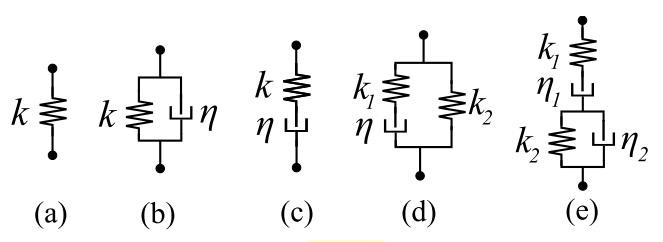
\includegraphics[width=0.6\textwidth]{HookeViscoelasticModels.PNG}
    \caption{Hooke's Law and linear viscoelastic models: (a) Hooke's Law (b) Kelvin-Voigt, (c) Maxwell, (d) Standard Linear Solid, and (e) Burger. The parameters $k$ and $\eta$ represent the spring stiffness and the dashpot viscous constant, respectively \cite{austin2015control}. }
    \label{fig:LinearViscoelasticModels}
\end{figure}

In line with the mentioned approach of relying on the controller to compensate the limitations of simple models, the work performed by Austin et al. modifies the viscoelastic Standard Linear Solid (SLS) model by implementing a piecewise linearization (PL) \cite{austin2015control}. The authors chose this model instead of the more complete, hence more complex, Burger model to keep the modeling process as simple as possible. The implementation of the PL method allowed the SLS model to account for the nonlinear properties of the material stress response. Due to this, the developed model is called the Standard Linear Solid model with Strain-Dependent Stiffness (Std. Lin. SDS). Nevertheless, the developed model was still unable to account for the material hysteresis, and, due to hardware limitations, the velocity-dependent stiffness effects were not validated. Moreover, experimental tests validated the changes on the material stiffness depending on the velocity of the applied deformation.

The PL method have proven to be a successful way to improve the prediction ability of traditional LVMs. Although it still has some limitations. The latter is addressed in this chapter by implementing the PL method in a more complex member of the LVMs, the Wiechert model. This is described in detail in \Cref{sec:wiechert}.

\section{The piecewise linearization method on the Wiechert model} \label{sec:wiechert}

The SLS model is frequently used when modeling viscoelastic materials, mainly due to its fairly simple mathematical model and its ability to account for creep and stress relaxation of the material (time-dependent properties). The SLS model can be viewed as a Maxwell model (also known as Maxwell branch) with an extra spring connected in parallel. The simplicity of the SLS model is also its main limitation. 
Viscoelastic materials are known to have more than one relaxation time, i.e. more than one Maxwell branch. In the linear viscoelastic models, the relaxation time depends on the viscous elements, i.e. dashpots. The Wiechert model, which is essentially a SLS model with $j$ Maxwell branches, is able to account for $j$ relaxation times and is illustrated in \Cref{fig:wiechert}. The time-dependent behavior of any viscoelastic material can be fully described by this model, given enough numbers of elements. However, the complexity of the model increases in proportion to the number of extra branches. Mathematically, each extra branch increases the derivative order of the model since more equations are required to account for the extra variables \cite{tirella2014strain,roylance2001engineering}.

\begin{figure}[hbt!]
	\centering
    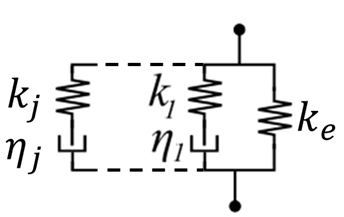
\includegraphics[width=0.3\textwidth]{WiechertModel.png}
    \caption{Wiechert Model. The components $k_1$, $\eta_1$, and the equilibrium spring $k_e$, together represents the SLS model. The components $k_j$, and $\eta_j$ represents the Maxwell Branch. The Wiechert model can contain as many branches as required, this is symbolised by the subscrip $j$. }
    \label{fig:wiechert}
\end{figure}

As previously described in \Cref{sec:viscoelasticity}, in addition to time-dependent and history-dependent properties, elastomers also have a nonlinear stress response. This can be partially described by the LVMs. The relaxation time constant of the dashpots in these models describes the nonlinear but time-dependent stress response of the material. Nonetheless, LVMs are not able to account for the strain-dependent response of materials. The latter is solved by the PL method as described in \cite{austin2015control}.

The spring in parallel with the other elements, in both the SLS model and the Wiechert model, is known as the equilibrium spring, and its stiffness $k_e$, is assumed constant. In reality, the stiffness $k_e$ of most elastomers is strain-dependent. 

Early attempts of modeling a strain-dependent stress response in viscoelastic materials are described by Schepelmann et al. in \cite{schepelmann2014compact}, where the stress-strain curve of a nonlinear rubber spring is approximated with an exponential model. In subsequent works, Austin et al. describes a piecewise linear regression fitted to the stress-strain curve of a material, in combination with the SLS model. 

The slope of the stress-strain curve represents the material's Young Modulus which is proportional to the material stiffness. During a tensile strength test the material is deformed at a constant rate, i.e. the stress response of the viscous element is also constant. Therefore, the observed nonlinear response is caused by the equilibrium spring.

Using the PL method, the nonlinear behavior of the equilibrium spring is approximated by considering it as several springs in parallel which ``engages" in sequence as the material strain increases. This is modeled by a summation of Heaviside functions centered in the desired strain in which each of the mentioned springs ``engages" and contributes with the total stress response of the material. In other words, the stress-strain curve of the material is segmented in several sections which relates a single stiffness to a strain range. This is illustrated in \Cref{fig:PLmethod}.

\begin{figure}[htb!]
	\centering
    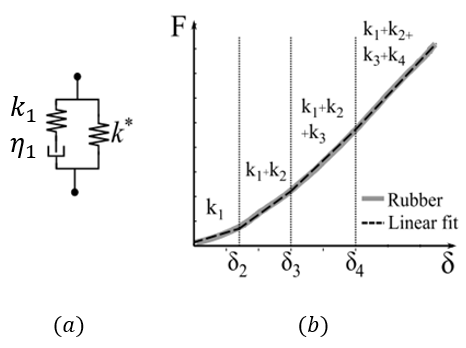
\includegraphics[width=0.6\textwidth]{PLmethod.png}
    \caption{(a) Standard Linearized Solid model with Strain-Dependent Stiffness. (b) Piecewise linearization method applied to the slope of the material load-displacement curve. This is analogous to many parallel springs which contribute to the material response depending on the material strain \cite{austin2015control}}.
    \label{fig:PLmethod}
\end{figure}

\subsection{Model fitting} \label{sec:Modelfit}

The mathematical expression for the SLS model and the Wiechert model can be simplified when considering a constant strain input (stress relaxation test). This simplification allows these models to be fitted into the stress relaxation curve and to approximate the parameter of interest, $k$ and $\eta$ \cite{roylance2001engineering}. The mathematical expression for the Wiechert model under a constant strain input is given by:

\begin{equation}
\label{eq1}
\sigma(t)=\Bigg\{k_e +  \sum_{j} k_j e^{-t/\tau_j}\Bigg\}\epsilon_o
\end{equation}

\noindent where $\sigma$ is the stress at a given time, $k_e$ is the equilibrium spring stiffness and $\varepsilon_o$ is the initial strain. For the summation, $\tau_j=\eta_j/k_j$ is the relaxation time constant, $k_j$ and $\eta_j$ are the spring stiffness and viscous constant of the elements in the $j^{th}$ Maxwell branch, respectively. For the specific case when $j = 1$, the resulting equation describes the SLS model under a constant strain input. In this case, the three parameters described in the SLS model: equilibrium spring stiffness $k_e$, dashpot viscous constant $\eta$ and the spring stiffness in the Maxwell branch $k_1$, can be obtained from the stress relaxation curve by analyzing three significant points: $t=0$, $t=\tau$, and $t=\infty$, as illustrated in \Cref{fig:stressTimeCurve}. The longer the duration of the test, the better the approximation of $k_e$.

\begin{figure}[htb!]
	\centering
    
\includegraphics[width=0.6\textwidth]{StressTimeCurve.png}
    \caption{SLS model fitted to a typical stress relaxation curve of a viscoelastic material. The parameters $k_e$, $k_1$ and $\eta$ can be obtained by analyzing three points in the curve: $t=0$, $t=\tau$, and $t=\infty$.}
    \label{fig:stressTimeCurve}
\end{figure}

The process to extract the parameters of the Wiechert model is more complicated due to its extra Maxwell branches, i.e. there are more than three points in time to be analyzed. These points can be selected using a collocation technique \cite{roylance2001engineering,machiraju2006viscoelastic}. In the reviewed literature, the points of interest are linearly scattered throughout the whole duration of the stress relaxation curve. Nevertheless, the decaying exponential term in \Cref{eq1} is better approximated by selecting the points of interest using a logarithmic scale. This is possible with the MATLAB function \texttt{logspace} which spreads evenly the desired number of points between the allowable decades. 
This is better described with the following example. A Wiechert model with six branches, $j=6$, wants to be fitted into a stress relaxation curve with four decades of duration ($t=10^4$ seconds). In total it would be required seven points in time, one for each branch and one for $t=0$. These points are spread as evenly as possible, using the total duration of the test, by the function \texttt{logspace}. The point $t=0$ is required for a correction described in the following paragraph. 

Similarly to the process illustrated in \Cref{fig:stressTimeCurve}, each point in time represents a time constant $\tau_j$ for which there is a known stress $\sigma_j$ from the experimental data. This can be rearranged into an equation system of $j$ equations with $k_j$ as the unknown variable as described in \cite{machiraju2006viscoelastic}. 

%Maybe bring the system of equations here?

Prior to this step, $k_e$ can be obtained using the equation for $\sigma(\infty)=\varepsilon_o k_e$, as illustrated in \Cref{fig:stressTimeCurve}. Subsequently, The Wiechert model in \Cref{eq1} can be completely described by solving the mentioned system of equations. Finally, after obtaining all the $k_j$, the value of $k_1$ is corrected, as described in \cite{roylance2001engineering}, by analyzing the point in time $t=0$.

The previous process allows the wiechert model equation to be fitted into the stress relaxation curve for a defined number of branches $j$. However, to obtain the optimal number of branches for each material, an iterative algorithm to find the smallest root mean square error (RMSE) between the Wiechert model response and the experimental data after testing different number of branches in the range of $j=[1,10]$ is implemented. The obtained optimal number of branches for each material varied between the range $j=[8,10]$. A higher number of branches has a meaningless improvement on the RMSE. Furthermore, beyond the number of branches $j=20$ the Wiechert model response shows an oscillatory behavior, hence a higher RMSE. Having obtained the parameters of interest for the SLS and the Wiechert model, their stress response under a constant strain is compared against the experimental data in Fig. \Cref{fig:StressRelFit}. 

\Cref{fig:StressRelFit} highlights the better accuracy delivered by the extra Maxwell branches in the Wiechert model in comparison to the simpler SLS model. As previously mentioned, \Cref{eq1} is a simplification helpful to approximate the parameters of both models but it is only applicable when the strain input is constant. The mathematical expression for the Wiechert model which describes the stress response under an unknown strain input, also called the constitutive equation can be found in \cite{roylance2001engineering}, in its Laplace. 
As previously mentioned, the Wichert model is an extension of the SLS model. Hence, when making $j=1$, the constitutive equation of the SLS model can be obtained, i.e. for an unkown strain input, is presented as follows:

\begin{figure}[htb!]
	\centering
    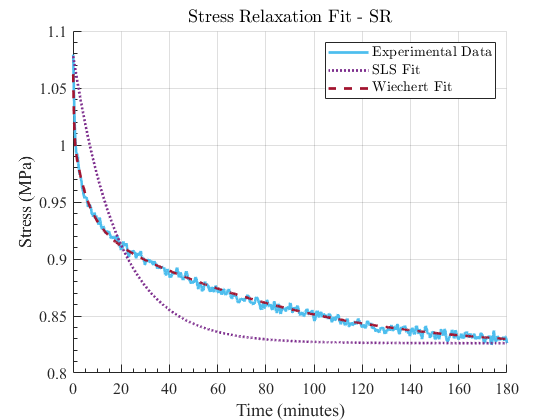
\includegraphics[width=0.93\textwidth]{SRelFit.png}
    \caption{Obtained fit from the Standard Linear Solid (SLS) and Wiechert model on the stress relaxation curve of the Silicone Rubber material. The obtained optimal number of branches of the Wiechert model fit is $j=8$.}
    \label{fig:StressRelFit}
\end{figure}

\begin{equation}
\label{eq3}
\dot{\sigma} + \frac{\sigma}{\tau_1} =  (k_e + k_1)\dot{\epsilon} + \frac{k_e\epsilon}{\tau_1}
\end{equation}

\noindent where $\epsilon$, $\dot{\epsilon}$, and $\dot{\sigma}$ are the strain, the strain rate and the stress rate, respectively (for the detailed procedure refer to \cite{roylance2001engineering}). Notice that the previous procedure will yield into a higher derivative order equation when applied to the Wiechert model due to its extra branches. A higher number of branches will increase the model accuracy at the cost of increasing its mathematical complexity. The constitutive equation of a Wiechert model with $j$ branches would result in a $j$ order differential equation similar to \Cref{eq3}. The aim of this chapter s to apply the PL method to the Wiechert model and evaluate its performance. Therefore, solving dealing with differential equations is out of the scope. Nonetheless, the Wiechert model can be evaluated by transforming it into a finite differences equation, as explained in \cite{roylance2001engineering}, yielding the following equation:

\begin{equation}
    \label{eq4}
    \sigma^t = k_e\epsilon^t + \sum_j \frac{k_j(\epsilon^t - \epsilon^{t-1}) + \sigma_j^{t-1}}{\bigg(1+\dfrac{\Delta t}{\tau_j}\bigg)}
\end{equation}

\noindent where the superscript $t-1$ and $t$ refers to values before and after a small time step $\Delta t$ have passed. Once again, making $j=1$ on \Cref{eq4} yields the finite difference version of the SLS model. The response of the two viscoelastic models of interest will be compared against the experimental data from the tensile strength test.

The next step in the fitting process focuses on the tensile strength test. In this test, the strain rate is constant, hence the resulting stress for both models (Fig. \Cref{fig:LinearViscoelasticModels}) is dependent on both the equilibrium spring and the Maxwell branches. At this stage of the model fitting, the parameters of the Maxwell branches in both models are known and their stress response can be calculated. The stress response of the equilibrium spring, $k_e$, can be isolated by subtracting the stress response of the Maxwell branches to the stress measured in the tensile strength test. 

After isolating the stress response of $k_e$, the final step in the fitting process is to implement the PL to both models and compare their response against the experimental data. Firstly, the stress-strain curve from tensile strength test is divided into $n$ segments. As previously explained, $k_e$ is considered as a group of parallel springs which ``engage" as the strain increases. This means, each subsequent stiffness is a combination of the ones found in previous segments of the stress-strain curve (Fig. \Cref{fig:PLmethod}).  Lastly, a linear regression is applied on the stress-strain curve for the desired $n$ strain segments to find the slope of the curve. This slope represents the stiffness of the equilibrium spring in each segment. By combining the $n$ obtained stiffness, the stress response of the strain-dependent stiffness $k_i^*$ is defined as follows:

\begin{equation}
\label{eq5}
\sigma^* = \sum_i^n k_i^* H_{\epsilon - \epsilon_i}(\epsilon - \epsilon_i)
\end{equation}

\noindent where $n$ is the desired number of strain intervals to fit, $\varepsilon_i$ represents the strain value at which the $i^{th}$ spring starts contributing to the stress response, the $H_{\epsilon - \epsilon_i}$ is the Heaviside or unitary step function centered at $\varepsilon_i$, i.e. the function output goes from 0 to 1 when $\varepsilon - \varepsilon_i = 0$. By substituting \Cref{eq5} into \Cref{eq3}, the Standard Linear Solid model with Strain-Dependent Stiffness is obtained \cite{austin2015control}.

Linear viscoelastic models describe a nonlinear relationship (decaying exponential time relaxation) between the applied strain and the resulting stress in a material. However, they only account for a linear stress response of the equilibrium spring. In reality, the relocation of internal molecular chains causes viscoelastic materials to exhibit a nonlinear and strain-dependent stress response. This can be solved by implementing the PL into \Cref{eq4}. The equilibrium spring stiffness $k_e$ is replaced by the strain-dependent stiffness $k_i^*$, yielding the linearized Wiechert model (PL-Wiechert) in \Cref{eq6}. Subsequently, the Std. Lin. SDS model, found in \cite{austin2015control}, is transformed into a finite difference equation, yielding \Cref{eq7}.

\begin{equation}
\label{eq6}
\sigma^t = \sigma^* + \sum_j \frac{k_j (\epsilon^t-\epsilon^{t-1}) + \sigma_j^{t-1}}{\bigg(1 + \dfrac{\Delta t}{\tau_j}\bigg)}
\end{equation}

\begin{equation}
\label{eq7}
\sigma^ t = \frac{1}{\bigg(1+\dfrac{\Delta t} {\tau_1} \bigg)} \Bigg[ \frac{\Delta t}{\tau_1} \sigma^* + (\sigma^* + k_1) (\epsilon^t-\epsilon^{t-1}) + \sigma^{t-1} \Bigg] 
\end{equation}

In this chapter, the linearized SLS model (\Cref{eq7}) is labelled as the piecewise linearized SLS (PL-SLS) model, differentiating it from the Std. Lin. SDS model documented in \cite{austin2015control} because the implemented fitting process is different. In here, the additional step of removing the stress response of Maxwell branches is performed. In summary, the experimental data from the stress relaxation test was used to obtain the parameters in the Maxwell branches of both models. The required number of branches was different per material, ranging from $j=8$ to $j=10$.  The constitutive equation of the Wiechert model was expressed as an equation of finite differences and subsequently linearized to obtain \Cref{eq6} (PL-Wiechert). Similarly, the constitutive equation of the SLS model, \Cref{eq3}, was modified in the same way, yielding \Cref{eq7} (PL-SLS).

\subsection{Findings}

At this stage of the research only six out of the seven soft materials previously mentioned were studied. The material missing in the following analyses is the Natural Rubber. Moreover, the stress-strain curves from the materials studied in this section are from the tensile strength test with 500 mm/min strain rate. With the exception of the Silicon Rubber material, for which the stress-strain curve for a strain rate of 50 mm/min was used. The complete list of the different tensile strength tests performed per material can be found in \Cref{tbl:tensile_tests}.

\subsubsection{Analysis of the optimal number of strain segments}

The amount of strain segments and their proper collocation have an impact on the PL method accuracy. In the work presented by Austin et al. there is no explanation of the criteria used to select the strain segments, only an illustration is provided \cite{austin2015control}. In this work, the variation of the slope in the stress-strain curve was used as the selection criteria. An optimization algorithm, which automatically collocates a new strain segment when the slope has varied outside a defined tolerance boundary, was developed.

The benefit of using this tolerance as the selection criteria for the number of strain segments to be created by the PL method, is two folds. On the one hand, the relationship between the number of strain segments and the desired tolerance is found to be exponential. On the other hand, the achievable RMSE for both models, in general for all materials, have minimal changes above a certain number of strain segments. In other words, beyond a certain number of strain segments, small improvements in the model accuracy requires a very large number of strain segments. This highlights a design trade-off between good accuracy and high computational complexity.

The PL-SLS model benefits the most from the PL method. It delivers a good accuracy even for small number of strain segments (\Cref{fig:SegmentsAll}). In contrast, the accuracy of the PL-Wiechert does not improve when using higher numbers of strain segments. Moreover, in the cases for the SR and EPR materials, the accuracy gets worse as the number of strain segments increases (\Cref{fig:SegmentsSR} and \Cref{fig:SegmentsEPR}).

The charts in \Cref{fig:SegmentsAll} are useful to select a proper value for the slope variation tolerance, taking into account the previously mentioned trade-off. It can be appreciated that the optimal tolerance is different for each material and dependent on the application. For the sake of analyzing the effect of the number of strain segments in the stress response of the PL-SLS and the PL-Wiechert models the tolerance value of 20\% is chosen. The obtained fit of both models is compared against the experimental data on \Cref{fig:ResponseAll}.

\begin{figure}[htb!]
    \centering
    \begin{subfigure}[b]{0.49\textwidth}
        \centering
        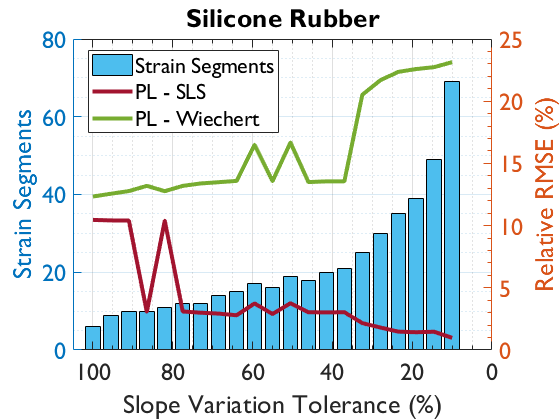
\includegraphics[width=\textwidth]{Segments_SR.png}
        \caption{}
        \label{fig:SegmentsSR}
    \end{subfigure}
    \begin{subfigure}[b]{0.49\textwidth}
        \centering
        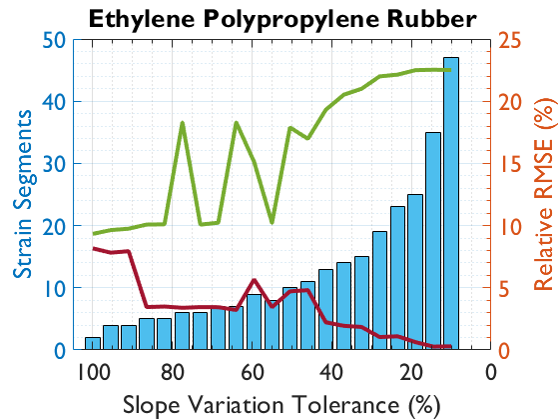
\includegraphics[width=\textwidth]{Segments_EPR.png}
        \caption{}
        \label{fig:SegmentsEPR}
    \end{subfigure}
    \begin{subfigure}[b]{0.49\textwidth}
        \centering
        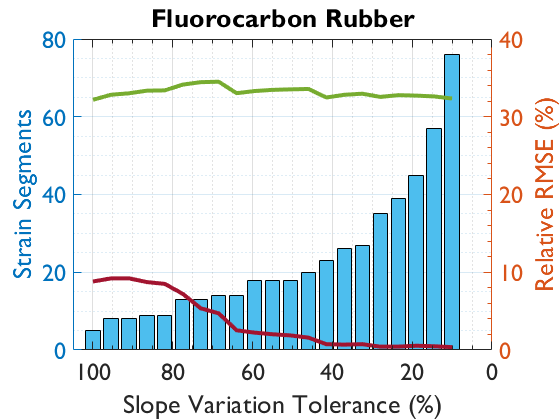
\includegraphics[width=\textwidth]{Segments_FR.png}
        \caption{}
        \label{fig:SegmentsFR}
    \end{subfigure}
    \begin{subfigure}[b]{0.49\textwidth}
        \centering
        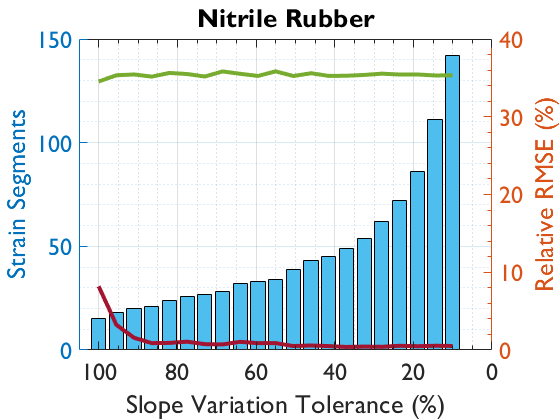
\includegraphics[width=\textwidth]{Segments_NR.png}
        \caption{}
        \label{fig:SegmentsNR}
    \end{subfigure}
    \begin{subfigure}[b]{0.49\textwidth}
        \centering
        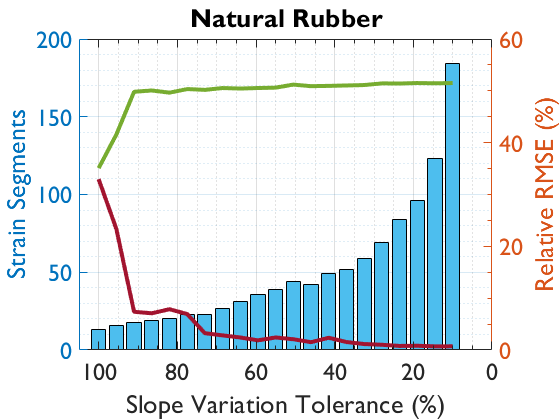
\includegraphics[width=\textwidth]{Segments_NatR.png}
        \caption{}
        \label{fig:SegmentsNatR}
    \end{subfigure}
    \begin{subfigure}[b]{0.49\textwidth}
        \centering
        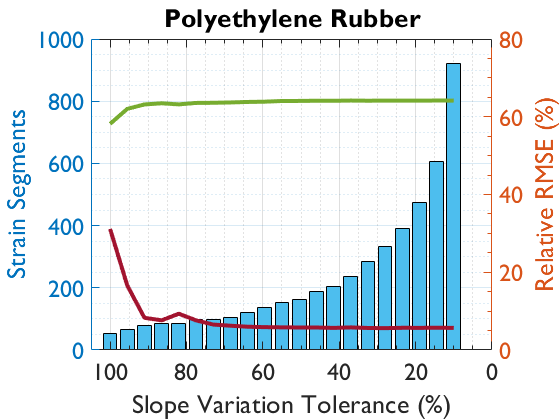
\includegraphics[width=\textwidth]{Segments_PR.png}
        \caption{}
        \label{fig:SegmentsPR}
    \end{subfigure}
    \caption{Relationship of the desired tolerance between the number of strain segments (blue bars), and the achievable rRMSE of the PL-SLS (solid red) and the PL- Wiechert (solid green) models, for all the soft materials (a-f). Figure taken from \cite{solis2018assessment}}
    \label{fig:SegmentsAll}
\end{figure}

\subsubsection{Analysis of model fit accuracy} \label{ModelfitAnalysis}

In general, the stress response from the PL-SLS model outperforms the response from the PL-Wiechert model (\Cref{fig:ResponseAll}). The PL-SLS model is able to accurately describe the stress-response of all the soft materials. Furthermore, it is able to achieve values of relative RMSE close to zero in four of the six rubber-based materials tested (\Cref{fig:SegmentsEPR,fig:SegmentsFR,fig:SegmentsFR,fig:SegmentsNR,fig:SegmentsNatR}). The slightly higher relative RMSE for the SR (\Cref{fig:SegmentsSR}) and PR (\Cref{fig:SegmentsPR}) materials might be caused by different factors, such as the incorrect selection of the stress relaxation test parameters, i.e. the initial strain $\varepsilon_o$ and the test duration. The PR material is unable to sustain high strains without suffering plastic deformation, even with this taken into account, an even smaller $\varepsilon_o$ is recommended. Another factor could be the time collocation method. The poor selection of the points in time to analyze can affect the accuracy of the parameters extracted. The logarithmic collocation approach used here yielded a large number of branches required to describe the material, which can cause the model response to oscillate.

In the case of the PL-Wiechert model, the very low obtained accuracy might be caused by an essential difference between \Cref{eq6} and \Cref{eq7}. In the latter equation, the strain-dependent stiffness $k_i^*$ interacts with the strain and the strain rate whereas in the former, $k_i^*$ only interacts with the strain. This lack of interaction of $k_i^*$ in the PL-Wiechert allow the abrupt step changes caused by the Heaviside function to disrupt the model stress response (\Cref{fig:ResponseEPR,fig:ResponseFR,fig:ResponseSR}).

\begin{figure}[htb!]
	\centering
    \begin{subfigure}[b]{0.49\textwidth}
        \centering
%\textwidth in this context is equal to the parent width
        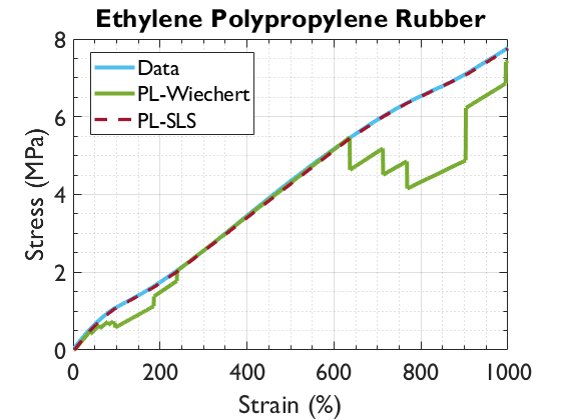
\includegraphics[width=\textwidth]{Response_EPR.png}
        \caption{}
        \label{fig:ResponseEPR}
    \end{subfigure}
    \begin{subfigure}[b]{0.49\textwidth}
        \centering
        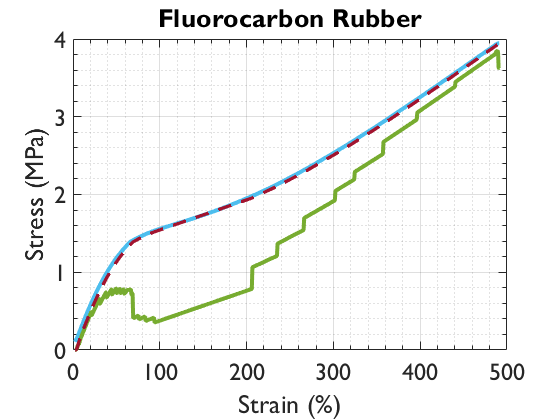
\includegraphics[width=\textwidth]{Response_FR.png}
        \caption{}
        \label{fig:ResponseFR}
    \end{subfigure}
    \begin{subfigure}[b]{0.49\textwidth}
        \centering
        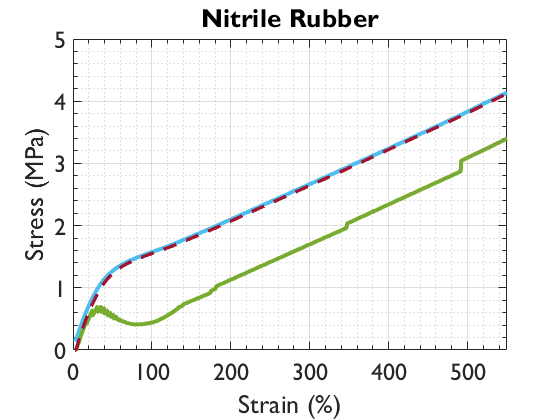
\includegraphics[width=\textwidth]{Response_NR.png}
        \caption{}
        \label{fig:ResponseNR}
    \end{subfigure}
    \begin{subfigure}[b]{0.49\textwidth}
        \centering
        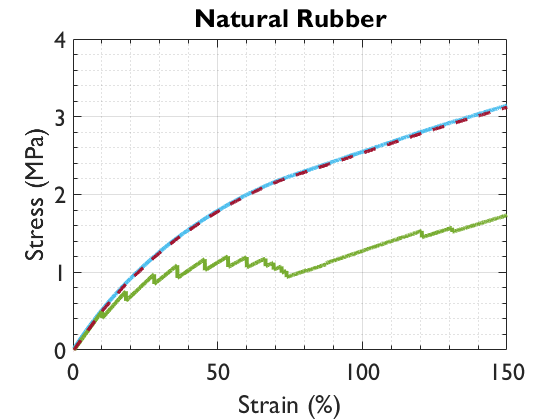
\includegraphics[width=\textwidth]{Response_NatR.png}
        \caption{}
        \label{fig:ResponseNatR}
    \end{subfigure}  
    \begin{subfigure}[b]{0.49\textwidth}
        \centering
        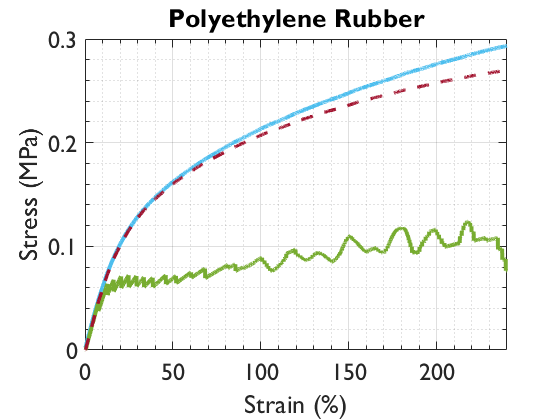
\includegraphics[width=\textwidth]{Response_PR.png}
        \caption{}
        \label{fig:ResponsePR}
    \end{subfigure}  
    \begin{subfigure}[b]{0.49\textwidth}
        \centering
        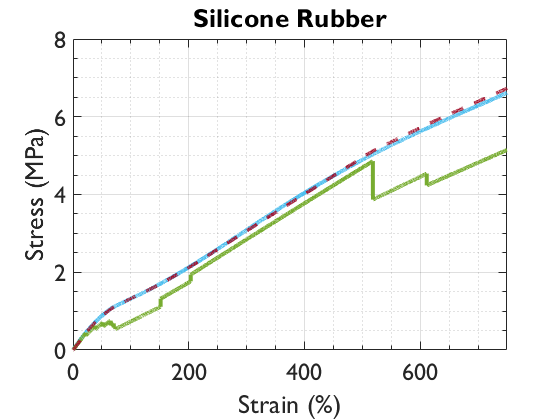
\includegraphics[width=\textwidth]{Response_SR.png}
        \caption{}
        \label{fig:ResponseSR}
    \end{subfigure}  
    \caption{Comparison between the experimental data from the Tensile Strength test and the stress response of the PL-SLS (dashed red) and the PL-Wiechert (solid green) models for all the soft materials (a-f). The number of strain segments required to meet the slope variation tolerance of 20\% for each material are EPR=20, FR=37, NatR=88, NR=73, PR=455 and SR=33. Figure taken from \cite{solis2018assessment}}
    \label{fig:ResponseAll}
\end{figure}

Nonetheless, the main limitation of the PL-SLS model is the inability to account the stress offset from the Maxwell branches. This was solved using the parameters obtained from the Wiechert model with $j$ branches, ultimately improving the stress response of the PL-SLS model. The PL-Wiechert model response can be improved by using its constitutive differential equation, similar to \Cref{eq3}. Even in its simplest form, i.e. $j=2$ the resulting second order differential equation might outperform the PL-SLS model due to the fact that the strain dependent stiffness $k_i^*$ will interact with different terms of the equation, providing that transforming it into a finite differences equation does not add extra complications.

Summarizing, in this section the design and development of two mathematical models for the prediction of the viscoelastic behaviour of soft materials is presented. On the one hand, the PL-SLS model, an optimized version of the documented Std. Lin. SLS model, is developed. On the other hand, the PL method was applied to the Wiechert model, a more complex LVMs. The results highlight the incompatibility of the PL method with a complex model such as the Wiechert model. However, the accuracy obtained by the developed PL-SLS is very promising. Hence, the PL-SLS model is used for further analyses.

\section{Accounting for the velocity-dependent stress response}

The PL-SLS model developed in here is based on the Std. Lin. SDS model, developed by Austin et al. \cite{austin2015control}. In their work, they were not able to test the ability of the developed model to account for the velocity-dependent stiffness on the studied material, due to hardware limitations. In this section, the latter is investigated by using the tensile strength data of seven soft materials under different strain rates. A total of three different strain rates were used in the tensile strength tests. Refer to \Cref{tbl:tensile_tests}, for the complete list of available datasets per material.

In the previous section, the capabilities of the PL-SLS model to predict the stress-response of the materials under a single strain rate were demonstrated. The main material parameter to extract from here is the strain-dependent stiffness of the equilibrium spring $k^*$. Looking back to the mechanical representation of the PL-SLS model in \Cref{fig:PLmethod}, it can be seen that the only time-dependent component is the dashpot located in the Maxwell branch. The relaxation time constant of this component was approximated using the stress relaxation test. Therefore, at this point, all the parameters from the PL-SLS model are known, i.e. all the parameters of the material are known.  

The PL-SLS model accuracy is exponentially proportional to the number of strain segments used. Previously, the relative RMSE was used as the parameter for measuring the performance of the model. Nonetheless, having a very small error does not necessarily reflect a good fit, and can in fact cause the fitted model to only perform well for a specific set of data, or in this case, a specific strain rate. Therefore, there must be an adequate number of strain segments which describes the strain-dependent stiffness of the materials under different scenarios, i.e. strain rates. The latter is investigated in this section.

The analysis performed in here consist as follows. The same stress-strain curves used in the previous section are used in here. That is, for the strain rate of 500 mm/min is used for all the materials, with the exception of the SR material, in which the stress-strain curve for a 50 mm/min strain rate is used. Subsequently, the PL-SLS model is fitted into these curves to extract the strain-dependent stiffness of the spring $k^*$. The latter is done for different tolerance values, ranging from 100 to 10, in steps of 10. Therefore, the fitting process is performed 10 times, i.e. 10 different $k^*$ are extracted. Then, the extracted $k^*$ are used to predict the stress-strain curve of the materials for all the other available strain rates (\Cref{tbl:tensile_tests}). The relative RMSE between the prediction of the PL-SLS model and the experimental data is calculated. Finally, the results are illustrated in \Cref{fig:GenAlmostAll,fig:GenOtherAll}.

In \Cref{fig:GenAlmostAll,fig:GenOtherAll} the performance of the PL-SLS to account for the velocity-dependent stress response of the materials is assessed. In general, there is not an immediate relationship between the tolerance values and the achieved relative RMSE. In some cases, using a lower tolerance value, hence fitting more strain segments to the stress-strain curve of the material, does improve the achieved relative RMSE (\Cref{fig:GenEPR,fig:GenNatPolR,fig:GenPR,fig:GenNatR2}). Moreover, the accuracy of the PL-SLS model decreases as the strain rate increases. This is very evident for the materials in which the stress-strain curve with the strain rate of 500 mm/min was used for the fitting process. In these cases, the PL-SLS model perform the worst for the stress-strain curve with the 50 mm/min strain rate (\Cref{fig:GenEPR,fig:GenFR,fig:GenNR,fig:GenNatPolR,fig:GenPR,fig:GenNatR1}). This is not as evident for the SR material, in which the stress-strain curve with strain rate of 50 mm/min was used. However, the relative RMSE does increase as the strain rate increase \Cref{fig:GenSR}. Furthermore, the performance of the PL-SLS model for the stress-strain curve with a 50 mm/min strain rate of the NatR material was found to be very poor (\Cref{fig:GenNatR1}). This could be caused by the low amount of data available for this specific strain rate. Therefore, this is considered as an isolated scenario.

\begin{figure}[htbp!]
	\centering
    \begin{subfigure}[b]{0.49\textwidth}
        \centering
        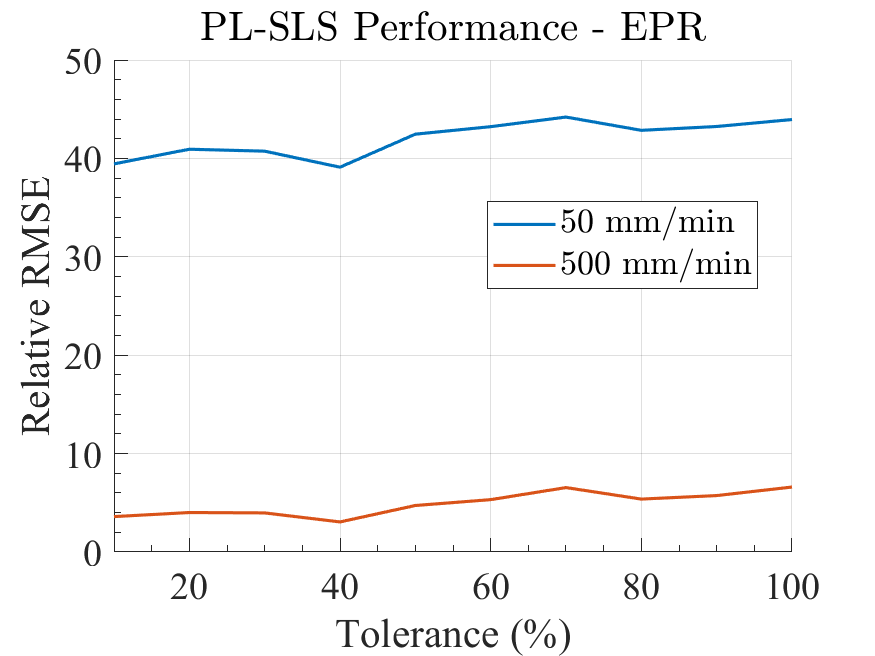
\includegraphics[width=\textwidth]{EPR_Generalization.png}
        \caption{}
        \label{fig:GenEPR}
    \end{subfigure}
    \begin{subfigure}[b]{0.49\textwidth}
        \centering
        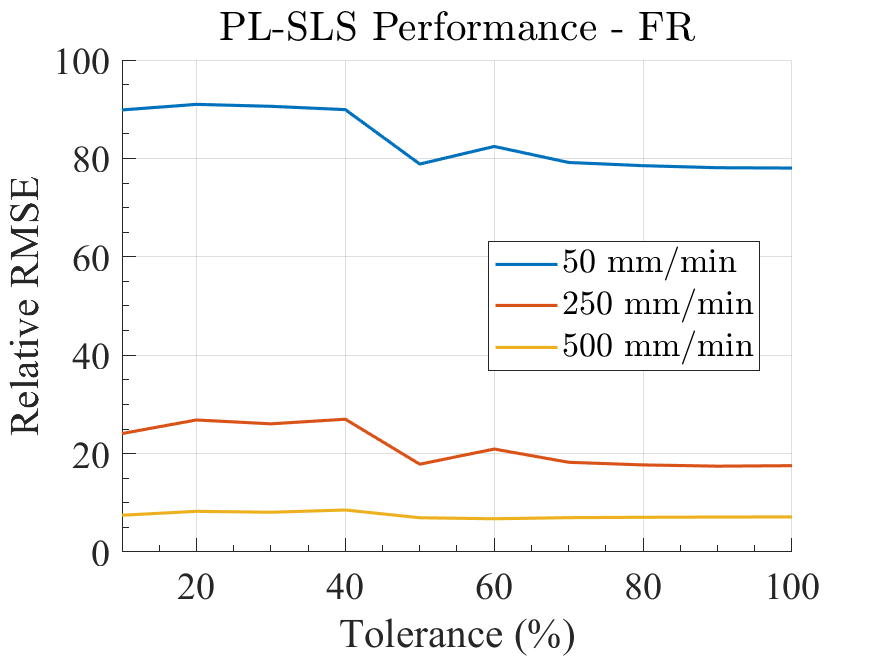
\includegraphics[width=\textwidth]{FR_Generalization.png}
        \caption{}
        \label{fig:GenFR}
    \end{subfigure}
    \begin{subfigure}[b]{0.49\textwidth}
        \centering
        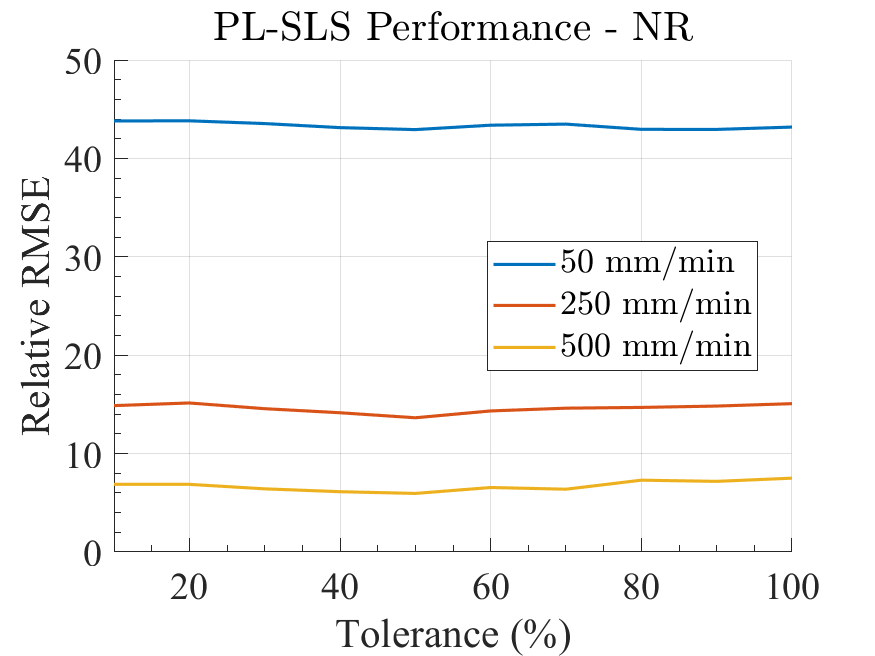
\includegraphics[width=\textwidth]{NR_Generalization.png}
        \caption{}
        \label{fig:GenNR}
    \end{subfigure}
    \begin{subfigure}[b]{0.49\textwidth}
        \centering
        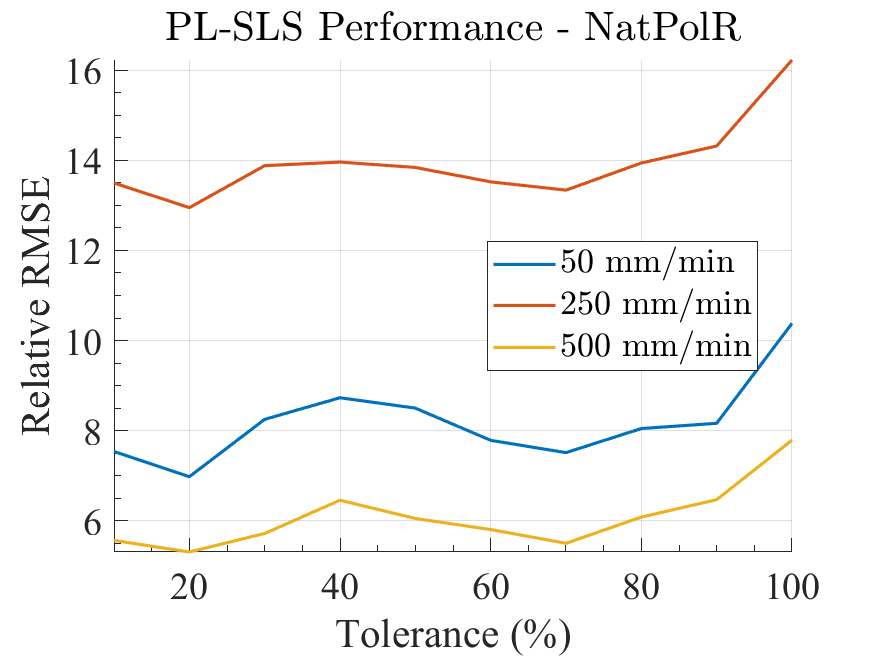
\includegraphics[width=\textwidth]{NatPolR_Generalization.png}
        \caption{}
        \label{fig:GenNatPolR}
    \end{subfigure}  
    \begin{subfigure}[b]{0.49\textwidth}
        \centering
        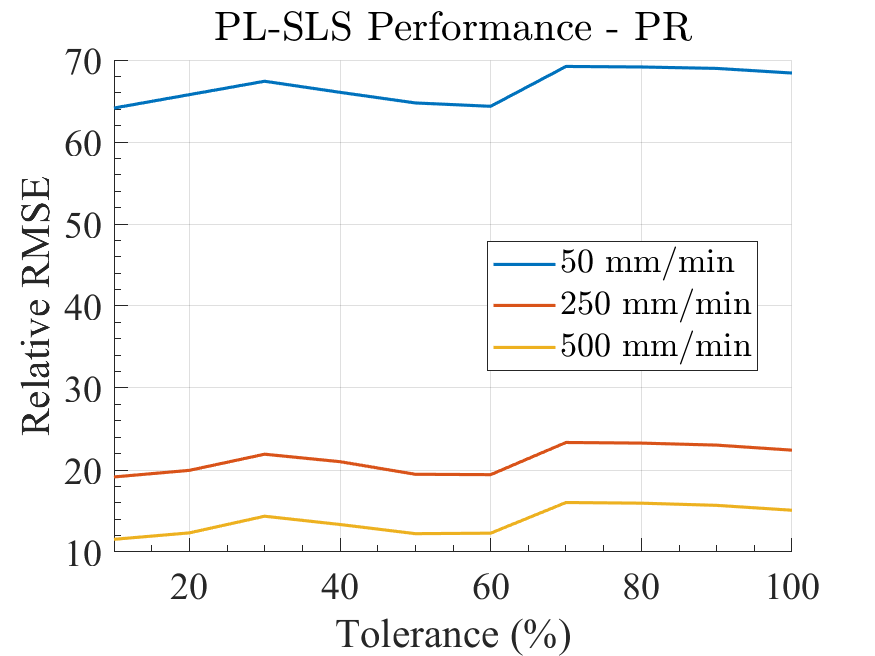
\includegraphics[width=\textwidth]{PR_Generalization.png}
        \caption{}
        \label{fig:GenPR}
    \end{subfigure}  
    \begin{subfigure}[b]{0.49\textwidth}
        \centering
        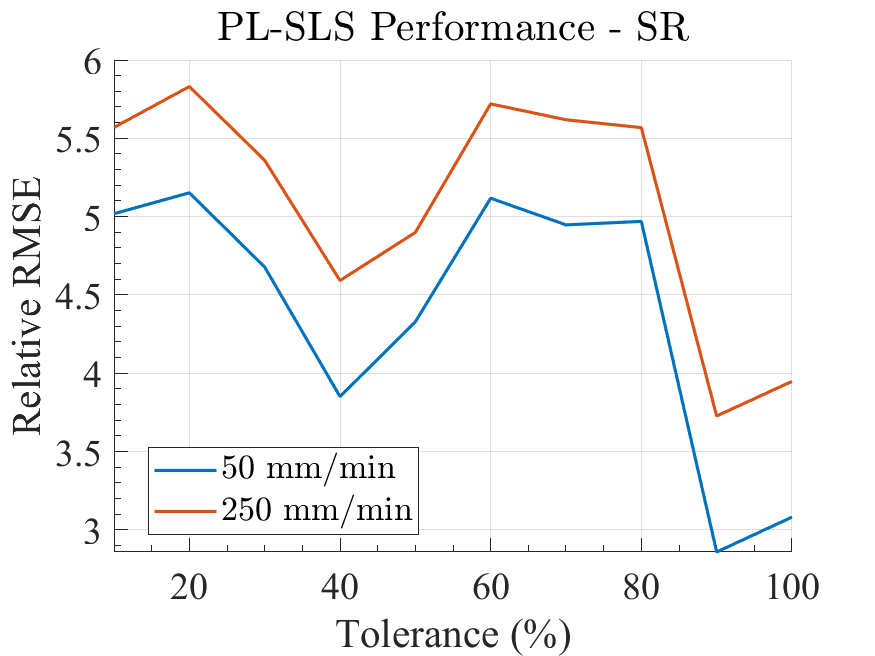
\includegraphics[width=\textwidth]{SR_Generalization.png}
        \caption{}
        \label{fig:GenSR}
    \end{subfigure}  
    \caption{Generalization capabilities of the PL-SLS model for the (a) EPR, (b) FR, (c) NR, (d) NatPolR, (e) PR and (f) SR materials. The strain dependent stiffness $k^*$ is fitted to the stress-stress curve of the materials for a 500 mm/min strain rate, using a range of 10 different tolerance values. With the exception of the SR material, in which the stress-strain curve from the 50 mm/min strain rate was used. Subsequently, the obtained $k^*$ is used to predict the stress-strain curve of the mentioned materials for other strain rates.}
    \label{fig:GenAlmostAll}
\end{figure}

\begin{figure}[htb!]
	\centering
    \begin{subfigure}[b]{0.49\textwidth}
        \centering
        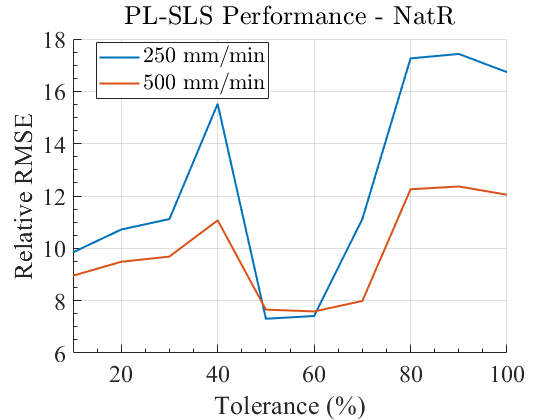
\includegraphics[width=\textwidth]{NatR2_Generalization.png}
        \caption{}
        \label{fig:GenNatR2}
    \end{subfigure}
    \begin{subfigure}[b]{0.49\textwidth}
        \centering
        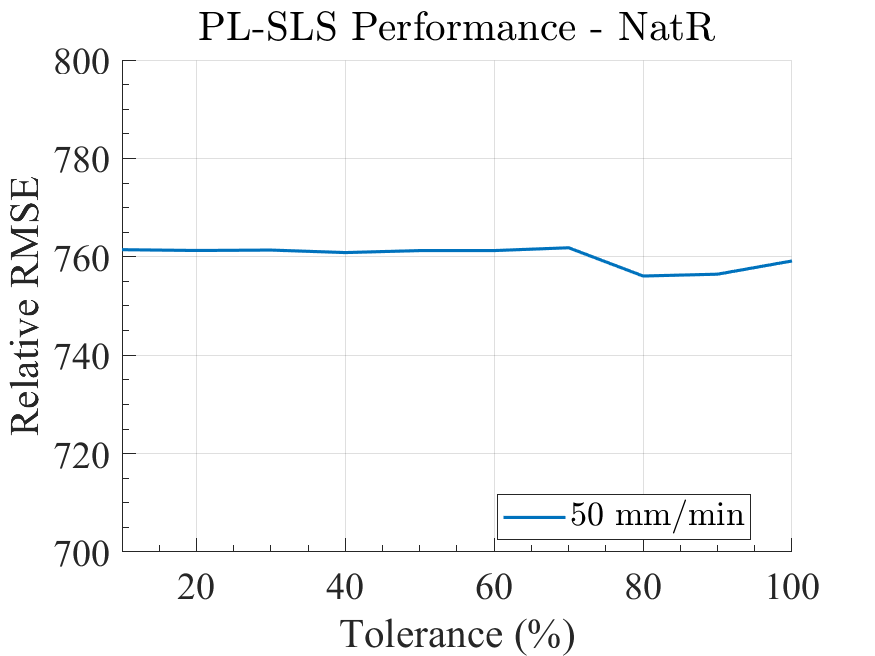
\includegraphics[width=\textwidth]{NatR_Generalization.png}
        \caption{}
        \label{fig:GenNatR1}
    \end{subfigure}
    \caption{Generalization capabilities of the PL-SLS model for the NatR material. The chart was divided into two due to the large difference in the achieved relative RMSE for the strain rate of (a) 250 mm/min and (b) 50 mm/min. The strain dependent stiffness $k^*$ is fitted to the stress-stress curve of the materials for a 500 mm/min strain rate, using a range of 10 different tolerance values. Subsequently, the obtained $k^*$ is used to predict the stress-strain curve of the mentioned materials for other strain rates.}
    \label{fig:GenOtherAll}
\end{figure}

In general, the PL-SLS model showed decent generalization capabilities for the NatPolR, SR and NatR materials, in which the highest relative RMSE obtained is below 20\% \Cref{fig:GenNatPolR,fig:GenSR,fig:GenNatR2}. Nonetheless, the PL-SLS model performed poorly for the remaining materials, as observed in \Cref{fig:GenEPR,fig:GenFR,fig:GenNR,fig:GenPR}, in which highest relative RMSE achieved is close to 100\%. Moreover, an example for the case in which the PL-SLS performed the worst and the best, are illustrated in \Cref{fig:WorstCase,fig:BestCase}, respectively.

As previously mentioned, the capabilities of the PL-SLS model to account for velocity-dependent (time-dependent) stress responses is thanks to the viscous element in the Maxwell Branches \Cref{fig:PLmethod}. Therefore, the performance of the PL-SLS model could be limited by the fact of only accounting for one time relaxation constant. In other words, the PL-SLS model is able to perform well for viscoelastic soft materials that are more on the elastic side than for those which have very strong viscous properties. The latter was one of the main motivations to analyze the Wiechert model as a potential alternative. However, this turned out to be unsatisfactory. The fact that the PL-SLS model performs well for soft materials with more dominant elastic properties means that the capabilities of accounting for velocity-dependent stress responses are poor.

\begin{figure}[htb!]
	\centering
    \begin{subfigure}[b]{0.49\textwidth}
        \centering
        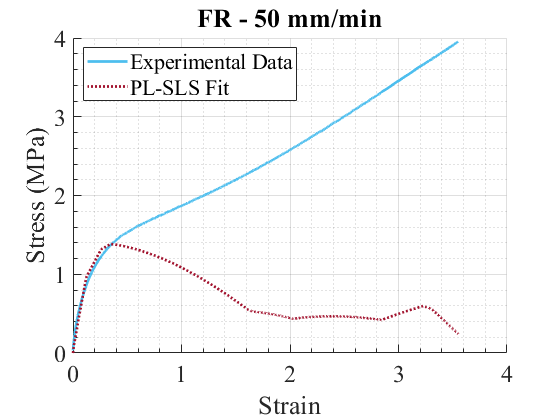
\includegraphics[width=\textwidth]{FR_WorstCase.png}
        \caption{}
        \label{fig:WorstCase}
    \end{subfigure}
    \begin{subfigure}[b]{0.49\textwidth}
        \centering
        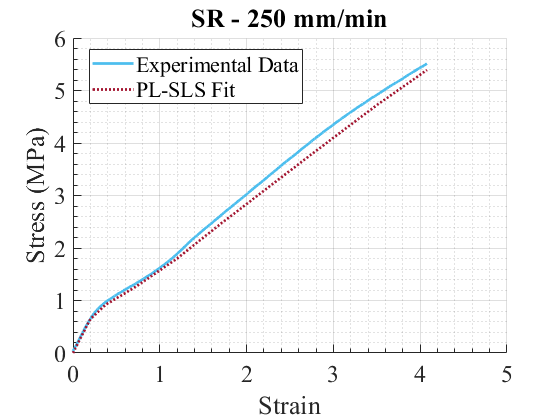
\includegraphics[width=\textwidth]{SR_BestCase.png}
        \caption{}
        \label{fig:BestCase}
    \end{subfigure}
    \caption{PL-SLS model prediction of a strain rate different to the one used in the fitting process. (a) Worst prediction performance case, for the FR material stress-strain curve with mm/min strain rate. (b) Best prediction performance case, for the SR material stress-strain curve with mm/min strain rate. The chosen tolerances values for (a) and (b), were 50\% and 10\%, respectively.}
    \label{fig:WorstBestCases}
\end{figure}

In conclusion, an in depth analysis of the elastic and viscous properties of the studied soft materials is not required to understand the main limitation of the PL-SLS model, which is not having more viscous components to account for more time relaxation constants. Nevertheless, the performed analysis highlighted the great potential of the PL-SLS model to describe the nonlinear and strain-dependent stress response of all the studied soft materials. Furthermore, the findings of the latter analysis indicate that there is little room left for making further optimizations to the developed model. Therefore, an alternative data-driven approach is investigated in the following sections of this research.


\section{Summary}

The experimental data obtained from the stress relaxation tests of six soft materials was used to describe the parameters of two mathematical models, the SLS and the Wiechert model. Both models were fit into the stress relaxation curve to extract their parameters. The fitting process for the SLS model is straight forward and the simplicity of the model yielded in a large RMSE. In contrast, the Wiechert model was fitted using a time collocation technique which yielded in a system of equations required to be solved to obtain all the model parameters. In addition, an optimization algorithm was implemented to obtain the right amount of Maxwell branches required to minimize the RMSE. The optimal number of branches varies from one material to the other in the range of $j=[8,10]$. The stress response of the optimal number of Maxwell branches was subtracted from the tensile strength test data. This step allowed the piecewise linearization to better approximate the strain-dependent stiffness of the equilibrium spring. Due to the lack of explicit information regarding the PL method implementation \cite{austin2015control}, an algorithm to locate the strain segments for the PL method using the variation of the slope of the stress-strain curve as the selection criteria, was developed. The relationship between the previous tolerance with the achievable relative RMSE and the number of strain segments was obtained (\Cref{fig:SegmentsAll}). These set of charts have the potential to be used as design guidelines when using the reported soft materials in robotic applications, since they highlight the trade-off between achievable accuracy and computational cost. The PL method was implemented into the linear viscoelastic models, obtaining the PL-Wiechert and PL-SLS models. These models were transformed into finite differences equations to evaluate their stress response. The obtained results demonstrated the great accuracy of the PL-SLS in describing the stress-strain curve of six soft materials. In contrast, implementing the PL method into a more complex viscoelastic model such as the Wiechert model, did not meet the expectations. The latter is due to an essential difference between \Cref{eq6} and \Cref{eq7}. In the latter equation, $k_i^*$ interacts with the strain and the strain rate whereas in the former, $k_i^*$ only interacts with the strain. This lack of interaction allows the abrupt step changes caused by the Heaviside function to disturb the PL-Wiechert model response.

The developed PL-SLS model, an optimized version of the Std. Lin. SDS model, was identified as the best candidate for the prediction of the nonlinear and strain-dependent stress response of the studied soft materials. In addition to this, the capabilities of the PL-SLS model to account for velocity-dependent stress responses was assessed. The latter analysis was not documented in the literature. The analysis yielded very interesting findings. On the one hand, the PL-SLS model is able to generalize well the stress-stain curves of the NatPolR, SR, and NatR materials, for up to three different strain rates. On the other hand, the PL-SLS model performed very poorly for the remaining materials. The poor performance of the PL-SLS model is directly related to the fact that the model only account for one time relaxation constant. In other words, the PL-SLS model is able to generalize well the stress response under different strain rate of viscoelastic soft materials which are more to the elastic side. Therefore, the model capabilities to account for velocity-dependent (time-dependent) stress responses is poor. Lastly, due to the latter findings, an alternative modelling tool is investigated in the following chapter.